\begin{tikzpicture}[x=0.48cm,y=0.43cm,thick]
  % Upper graph: y=c-sin(t), with c=1/2 and two adjacent roots marked.
  \draw[->] (-5.9,0)--(13.9,0) node[right] {$t$};
  \draw[->] (0,-1.5)--(0,1.75) node[above] {$y$};
  \draw[domain=-5.8:13.8,samples=220,smooth,variable=\t] plot (\t,{0.5-sin(57.2958*\t)});
  \fill (0.524,0) circle (1.4pt) node[below] {$r_1$};
  \fill (2.618,0) circle (1.4pt) node[below] {$r_2$};
  \node at (9.6,-1.05) {$y=c-\sin t$};
  % Reciprocal branches; vertical dashed lines are singular times.
  \begin{scope}[yshift=-5.0cm]
    \draw[->] (-5.9,0)--(13.9,0) node[right] {$t$};
    \draw[->] (0,-3.1)--(0,3.1) node[above] {$y$};
    \foreach \a in {-5.76,0.524,6.807,13.091} {\draw[dashed,thin] (\a,-3.05)--(\a,3.05);}
    \foreach \a in {-3.665,2.618,8.901} {\draw[dashed,thin] (\a,-3.05)--(\a,3.05);}
    \draw[domain=-5.70:-3.72,samples=100,smooth,variable=\t] plot (\t,{max(-3,min(3,1/(0.5-sin(57.2958*\t))))});
    \draw[domain=-3.60:0.45,samples=120,smooth,variable=\t] plot (\t,{max(-3,min(3,1/(0.5-sin(57.2958*\t))))});
    \draw[domain=0.60:2.55,samples=100,smooth,variable=\t] plot (\t,{max(-3,min(3,1/(0.5-sin(57.2958*\t))))});
    \draw[domain=2.70:6.75,samples=120,smooth,variable=\t] plot (\t,{max(-3,min(3,1/(0.5-sin(57.2958*\t))))});
    \draw[domain=6.90:8.85,samples=100,smooth,variable=\t] plot (\t,{max(-3,min(3,1/(0.5-sin(57.2958*\t))))});
    \draw[domain=8.97:13.0,samples=120,smooth,variable=\t] plot (\t,{max(-3,min(3,1/(0.5-sin(57.2958*\t))))});
    \node at (10.9,-4.20) {$y=\dfrac{1}{c-\sin t}$};
    \fill (0.524,0) circle (1.4pt) node[below] {$r_1$};
    \fill (2.618,0) circle (1.4pt) node[below] {$r_2$};
  \end{scope}
\end{tikzpicture}
